\chapter{Визначення метрологічних характеристик використаних приладів}
\section{Визначення метрологічних характеристик електроного ємнісного гігрометра}

Для визначення метрологічних характеристик ємнісного гігрометра було використано
зразковий (еталонний) гігрометр ``Testo 605 H1'' і мультиметр налаштований на вимірювання ємності який
було під’єднано до досліджуваного гігрометра.

Отримано 11 значень вологості і напруги. Результати обрахунків та вимірювань наведені в таблиці \ref{t:metrological_exp}

\input{./py/print_sensitivity_table.tex}

\subsection{Визначення чутливості кожного з результатів}

Знайдемо чутливість для кожного з результатів:

\begin{equation}
  S = \frac{C}{\varphi}
\end{equation}

\begin{itemize}
\item [Де:] $C$ --- ємність мембрани, ~пФ;
\item []$\varphi$ ---  значення вологості, ~\%.
\end{itemize}

\input{./py/print_sensitivity.tex}


\subsection{Визначення середньої чутливості}

 Розрахуємо середню чутливість:

 \begin{equation}
   S_{\text{ср}} = \frac{\sum S_n}{n}
 \end{equation}

 \begin{itemize}
 \item [Де:] $S_n$ --- чутливість n-го результату спостереження, пФ/\%;
 \item []$n$ ---  кількість результатів спостереження.
 \end{itemize}

 \input{./py/print_sensitivity_am.tex}


\subsection{Визначення cумарної середньої квадратичної похибки вимірюваня}

\begin{equation}
  \Delta C_{\sum} = \sqrt{\Delta C_1^2 + \Delta C_2^2}
\end{equation}

\begin{equation}
  \Delta \varphi = \frac{\varphi_{max} \cdot \gamma_{\text{гігр.}} }{100}
\end{equation}
\begin{itemize}
\item [Де:] $\varphi_{max}$ --- максимальне значення вологості, \%;
\item []$\gamma_{\text{гігр.}}$ ---  приведена похибка гігрометра.
\end{itemize}

\begin{gather}
  \varphi_{max} = 95 ~\%; \nonumber\\
  \Delta \gamma_{\text{гігр.}} = 1 ~\%; \\
  \Delta \varphi = \frac{95 \cdot 1}{100} = 0.95 \%. \nonumber
\end{gather}
\begin{equation}
    \Delta C_1 = \Delta \varphi \cdot S_{\text{cep}} = 0.95 \cdot 8.14 = 7.73 ~\text{пФ}
\end{equation}
\begin{gather}
    C_{max} = 2000 ~\text{пФ}; \nonumber\\
    \Delta \gamma_{\text{мульт.}} = 1 ~\%; \\
    \Delta C_2 = \frac{C_{max} \cdot \gamma_{\text{мульт.}}}{100} = \frac{2000 \cdot 1}{100} = 20 ~\text{пФ}. \nonumber
\end{gather}

\begin{equation}
  \Delta C_{\sum}  = \sqrt{23.16^2 + 20^2} = 83.285 ~\text{пФ}
\end{equation}

\subsection{Визначення приведеної похибки вимірювання}
Визначимо приведену похибку:

\begin{equation}
    \delta_{\sum} = \frac{\Delta C_{\sum}}{C_i}
\end{equation}
\begin{itemize}
\item [Де:] $\Delta C_{\sum}$ --- сумарна середня квадратична похибка вимірювання, пФ;
\item []$C_i$ ---  i-й результат спостереження.
\end{itemize}
\input{./py/print_delta_sum.tex}

\subsection{Визначення відносної похибки вимірювання}
Визначимо відносну похибку вимірювання за наступною формулою:
\begin{equation}
    \gamma_{\sum} = \frac{\Delta C_{\sum}}{C_{\text{макс}}} \cdot 100\%
\end{equation}
\begin{itemize}
\item [Де:] $\Delta C_{\sum}$ --- сумарна середня квадратична похибка вимірювання, пФ;
\item []$C_{\text{макс}}$ ---  максимальне значення ємності.
\end{itemize}
\begin{equation}
    \gamma_{\sum} = \frac{21.443}{2000} \cdot 100\%= 1.07\%
\end{equation}

\subsection{Визначення варіації}
\begin{equation}
    b_4 = |452 - 450| = 2~\text{пФ}
\end{equation}
\subsection{Статична характеристика}

Графік статичної характеристики наведено на \ref{fig:static_c}

\begin{figure}[htb]
\centering{
\resizebox{\textwidth}{!}{
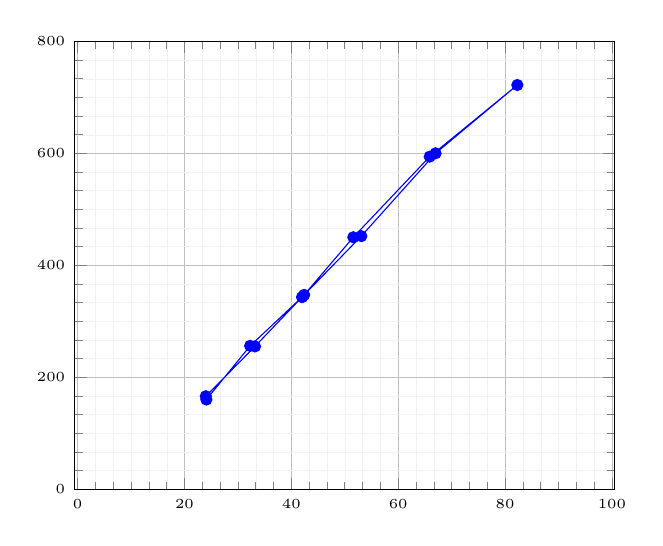
\begin{tikzpicture}
\begin{axis}[
    xmin=0,
    xmax=100,
    ymin=0,
    ymax=800,
    grid=both,
    grid style={line width=.1pt, draw=gray!10},
    major grid style={line width=.2pt,draw=gray!50},
    minor tick num=5,
    enlargelimits={abs=0.5},
    axis line style={latex-latex},
    ticklabel style={font=\tiny,fill=white},
]

\addplot[
    color=blue,
    mark=*,
    ]
    coordinates {
    (24.1, 160)(32.3, 256)(42.0, 343)(53.1, 452)(67.0, 600)(82.3, 722)(65.9, 594)(51.6, 450)(42.4, 347)(33.2, 255)(24.0, 166)
    };

\end{axis}
\end{tikzpicture}}}
\caption{Статична характеристика}
 \label{fig:static_c}
\end{figure}
\newpage
\section*{Висновки до розділу 3}
\addcontentsline{toc}{section}{Висновки до розділу 3}

Визначено метрологоічні характеристики електронного ємнісного гігрометра ``Testo 605 H1'', проведено
ознайомелення з методикою повірки метрологічних приладів.
